\section{Patientgruppe}
\textit{Følgende afsnit omhandler omfanget af lidelsen, knæartrose. Afsnittet redegør for patientomfanget, samt de forskellige disponeringsfaktorer, sammenkoblet med lidelsen. Ydermere vil patienternes patientforløb blive redegjort, hvoraf den sidste fase vil blive analyseret. Ovenstående vil danne grundlag for at klassificere en patientgruppe til knæalloplastik.}

Knæartrose er en lidelse der gradvist nedbryder knæets ledbrusk, hvorefter der kan forekomme forandringer i leddets knogler. Disse deformationer er irreversible, hvormed knæartrose kun afhjælpes og ikke kurreres. Lidelsen kan opdeles i en primær- og sekundær artrose. Den primære artrose er bestående af ikke-udefrakommende årsager, hvilket indebærer genetik samt aldring. Den sekundære artrose indebærer tidligere skader, sygdom, inflammation, overvægt samt traume. Knæartrose er en tilstand hvis hyppigste symptomer er smerter samt nedsat mobilitet hos den påvirkede. Smerterne udtrykkes i forskellig grad, fra igangsættende smerte til kronisk tilstedeværende smerte. Generelt for knæartrose, forværres symptomerne i takt med graden af lidelsen øges. \citep{Lind2016b}

En længere række faktorer har betydning for udviklingen af artrose. Hvis en eller flere af disse faktorer er tilstede, er den påvirkede mere disponeret for knæartrose. Dette er eksempelvis, overbelastning igennem arbejde og fritid, tidligere knæskader, genetisk arv, overvægt samt køn \citep{brostrom2012}. Knæartrose er til stede blandt 45\% af alle 80-årige af befolkningen. Dette kan formodes at stige da levealderen i Danmark stiger. Dette er ikke det eneste faktor hvorfor prævalensen kan antages at stige. En af risikofaktorerne for udviklingen af knæartrose er overvægt, hvilket 47\% af den danske befolkning kan kategoriseres som. Ydermere stiger andelen af overvægtige med alderen, hvilket ligeledes er tilfældet for knæartrose. Overvægtige er disponeret for knæartrose med en relativ risiko på en faktor tre, hvoraf en kombination af ovenstående faktorer øger risikoen for lidelsen. \citep{Vestergaard2014} \citep{Vestergaard2016} \citep{Lind2016} \citep{Lind2016b}

En patients symptomer kan medføre igangsættelsen af et behandlingsforløb. Et behandlingsforløb for en patient med knæartrose består af flere faser, hvis mål er smertelindring, mobilitetsforøgelse samt forebyggelse. Generelt kan faserne opdeles i ikke-invasive og invasive metoder. Hvilken metode som hjælper patienten afhænger graden af knæartrose.

\begin{figure}[H]
	\centering
	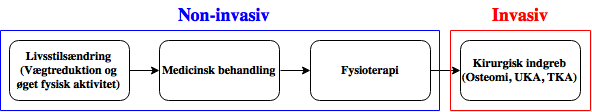
\includegraphics[width=1\textwidth]{figures/bProblemanalyse/flowchart_behandlingsforloeb.png}
	\caption{På figuren ses et flowchart indeholdende de forskellige behandlingsmetoder der forekommer igennem et patientforløb med knæartrose.}
	\label{fig:flow_behandlingsfaser}
\end{figure}\vspace{-.25cm}

Som det ses på \figref{fig:flow_behandlingsfaser}, består første fase, hvis nødvendig, af en livsstilsændring, hvor en vægtreduktion samt øget fysisk aktivitet uden belastning, kan afhjælpe patients symptomer. Hvis dette ikke er tilstrækkeligt kan medicinsk behandling i form af smertelindrende medikamenter benyttes, enten som enkeltstående behandling eller sideløbende med fysioterapi. Hvis ikke, de non-invasive behandlingsmetoder afhjælper lidelsen i en grad hvor patienten er tilfreds, så bliver de invasive behandlingsmetoder taget til overvejelse. Overvejelsen heraf indebærer den diagnosticerede grad af artrose, hvilket består af en sammenkobling af den kliniske vurdering, verificeret med forandringer i knæet opnået gennem røntgenbilleder. Baggrunden for at den kliniske vurdering skal verificeres forud for kirurgi, er at smerte fra hofte og ryg, kan projiceres til knæet. Resultatet heraf er at patienten først berettiget kirurgi og hermed en total knæalloplastik (TKA), når non-invasive behandlingsmetoder ikke har haft tilstrækkelig effekt. Ydermere skal patienten besidde moderat til svær artrose for at kvalificeres til kirurgi. \citep{Lind2016b} \citep{brostrom2012} \citep{skou2016}

TKA er den sidst mulige behandlingsmetode for at lindre patientens symptomer vedrørende knæartrose. Dette resulterede i at der i 2014 blev udført omtrent 9.800 TKA operationer, fordelt på førstegangs- og revisions operationer. \citep{aarsrapport2016} Idet TKA er den sidste behandlingsmulighed, er operationstilfredshed en betydningsfuld problematik. I 2012 viste en undersøgelse fra Sundhedsstyrelsen, at 81-85\% af patienter der havde modtaget en TKA operation tilfredse, 8-11\%var decideret utilfredse, og resten var i tvivl eller til dels utilfreds. Dette er ensbetydende med at der potentielt er 19\% af alle operationer fra et patientøjemed som ikke er succesfulde. Resultatet heraf er at op mod 19\% ikke opnår bedring fra deres smerter samt eventuel nedsat mobilitet. \citep{brostrom2012} \cite{Sakellariou2016} har lavet en risikovurdering vedrørende kroniske smerter efter TKA. Udfra resultaterne viste \cite{Sakellariou2016}, at op mod 39\% af studiets patienter oplevede moderat til alvorlig smerte, et år postoperativt TKA. Ifølge International Association for the Study of Pain (IASP) defineres kroniske smerter, som tilstedeværende smerter efter tre måneder. \citep{Sakellariou2016} \\
Patientgruppen som postoperativt ikke er tilfredse er svært definerbar. Problematikken opstår i og med klassificeringen bag de potentielt 19 til 39~\% utilfredse patienter er vedrørende postoperative smerte samt mobilitet. Det kan forestilles at der blandt patienterne findes en forventningsfaktor, hvilket gør de kan kategoriserer dem selv som værende utilfreds, omend de rent faktisk har opnået en forbedring af både smerte og eller mobilitet. Det kan tænkes at forventningsfaktoren kan være medvirkende til kategorisere dem som værende utilfredse, som resultat af skuffelsen af ikke at fungere som et individ med et fuldt funktionsdygtigt knæ.  

Knæartrose er som følge af samfundets udvikling, en lidelse i vækst da den umiddelbare disponerede målgruppe er voksende. Resultatet heraf medfører at antallet af registrerede tilfælde med symptomer sandsynligvis ligeledes vil stige, og der vil forekomme flere patienter med kroniske smerter postoperativt TKA, uden mulighed for yderligere alternativ behandling.

